\documentclass[12pt]{article}

\usepackage{geometry}
\geometry{margin=1in}
\usepackage{amsmath, amssymb}
\usepackage{graphicx}
\usepackage{hyperref}
\hypersetup{colorlinks=true, linkcolor=black, citecolor=black, urlcolor=blue}
\usepackage{listings}
\usepackage{xcolor}
\usepackage{booktabs}
\usepackage{caption}
\usepackage{float}
\usepackage{parskip}
\usepackage{microtype}

\definecolor{codebg}{RGB}{245,245,245}
\definecolor{codeframe}{RGB}{200,200,200}
\definecolor{codecomment}{RGB}{90,110,90}
\definecolor{codekw}{RGB}{0,80,180}
\definecolor{codestr}{RGB}{160,30,30}

\lstdefinestyle{pythonstyle}{
    backgroundcolor=\color{codebg},
    frame=single,
    rulecolor=\color{codeframe},
    basicstyle=\ttfamily\footnotesize,
    keywordstyle=\color{codekw}\bfseries,
    commentstyle=\color{codecomment}\itshape,
    stringstyle=\color{codestr},
    breaklines=true,
    numbers=left,
    numberstyle=\tiny\color{gray},
    numbersep=8pt,
    language=Python,
    showstringspaces=false,
    tabsize=4,
    captionpos=b
}
\lstset{style=pythonstyle}

\title{\textbf{Geometric Steganography via Angular Encoding\\
of Color Vectors in Cover Images}}

\author{
    Mahanti Pranith \\
    Department of Computer Science \\
    BITS Pilani, Hyderabad Campus \\
    \texttt{pranithmahanti@gmail.com}
}

\date{}

\begin{document}

\maketitle

\begin{abstract}
We present a steganographic method that embeds textual messages into
existing cover images by rotating the color vectors of selected pixels to
target directions in the RG plane, leaving pixel magnitudes and the B
channel unchanged. Each of 37 character tokens is assigned a unique angular
sector of approximately $9.73°$; encoding a token rotates the
$(R{-}128,\,G{-}128)$ vector of the corresponding cover pixel into that
sector while preserving the vector's original Euclidean length. We give a
complete implementation, derive the quantization error bounds that govern
decoding accuracy, and evaluate the scheme with respect to three criteria:
decoding fidelity, perceptual distortion (PSNR and per-pixel Euclidean
distance), and statistical detectability via angle-histogram and
polar-distribution analysis. The encoding introduces a characteristic
37-spoke angular signature absent from natural images and detectable by
straightforward statistical tests. Two principled extensions are proposed
to address this: a differential scheme that accumulates angular increments
and eliminates the fixed-spoke signature, and a spherical generalization
that exploits all three color channels to increase capacity and reduce
detectability.
\end{abstract}

% ─────────────────────────────────────────────────────────────────────────────
\section{Introduction}
\label{sec:intro}

Steganography hides a message inside a carrier medium so that an observer
cannot detect its presence. The carrier must be independently plausible; a
randomly generated image reveals the act of concealment regardless of how
well the message is hidden within it. This distinguishes steganography from
mere encoding: the cover object must exist as a natural artifact before
any message is embedded \cite{simmons1984prisoners}.

Classical image steganography operates either in the spatial domain, by
modifying pixel intensity values, or in a transform domain, by modifying
frequency coefficients. The canonical spatial method is Least Significant
Bit (LSB) substitution \cite{johnson2001steganography}: the lowest-order
bit of each color channel is overwritten with one bit of the secret message.
The modification is imperceptible because a change of $\pm1$ in a pixel
value on the range $[0, 255]$ lies below the human visual threshold, yet it
is statistically detectable because it disturbs the characteristic
value-pair statistics of natural images \cite{fridrich2001detecting}.

We explore an orthogonal approach grounded in a geometric observation: the
RGB triple of a pixel can be interpreted as a vector in three-dimensional
color space. Conventional steganography modifies the magnitude of individual
components; we instead encode information in the vector's direction while
preserving its magnitude. This is directly analogous to phase-shift keying
in communications, where data is carried in the phase of a carrier signal
rather than its amplitude \cite{johnson2001steganography}.

Concretely, we center each pixel at the gray point $(128, 128, 128)$ and
treat the $(R{-}128,\,G{-}128)$ pair as a 2D vector in the RG plane. To
embed a character token, we rotate this vector to the angular sector
assigned to that token while preserving the vector's Euclidean length and
leaving the B channel unmodified. The result is a stego image that is
visually similar to the cover image and whose pixel values have been altered
in a geometrically structured way.

The contributions of this paper are:
\begin{itemize}
    \item A complete cover-image steganographic scheme based on angular
          encoding in the RG plane, with a magnitude-preservation strategy
          that minimizes brightness distortion.
    \item A rigorous quantization error analysis that characterizes when
          decoding succeeds and fails as a function of pixel magnitude.
    \item An experimental evaluation comparing cover and stego images across
          four metrics: angle-histogram shift, polar distribution, per-pixel
          distortion, and PSNR.
    \item A characterization of the geometric fingerprint introduced by
          encoding, and two proposed extensions designed to eliminate it.
\end{itemize}

% ─────────────────────────────────────────────────────────────────────────────
\section{Related Work}
\label{sec:related}

\subsection{Spatial Domain Steganography}

LSB substitution replaces the least significant bit(s) of pixel channel
values with message bits \cite{johnson2001steganography}. A change of
$\pm1$ is perceptually invisible but statistically detectable: Fridrich
et al.\ \cite{fridrich2001detecting} showed that LSB embedding disturbs
the histogram of value pairs in a characteristic pattern detectable by
RS analysis and pairs analysis. LSB matching improves on direct
substitution by randomly incrementing or decrementing the pixel value
when the LSB already matches the message bit, flattening the pair
histogram at the cost of increased overall noise.

\subsection{Transform Domain Steganography}

F5 \cite{westfeld2001f5} embeds data in the DCT coefficients of JPEG
images using matrix embedding to minimize the number of modified
coefficients. Transform-domain methods are more robust to post-processing
than spatial-domain methods but are constrained to specific file formats
and cannot operate on losslessly stored images without first computing a
transform.

\subsection{Phase Encoding}

Phase encoding for audio steganography replaces the initial phase of DFT
segments with a target phase while preserving magnitude
\cite{johnson2001steganography}. The human auditory system is substantially
less sensitive to phase than to magnitude, making this approach
low-distortion. Our method adapts the same philosophy to the color domain:
vector magnitude is treated as a perceptually significant quantity to be
preserved, while direction carries the message.

\subsection{Position of This Work}

Unlike LSB methods, our scheme modifies directional properties of color
vectors rather than their intensity values. Unlike transform-domain methods,
it operates directly in the spatial domain of a natural cover image with no
frequency transform. To our knowledge, directional encoding of color vectors
in the RG subspace of natural images has not been previously characterized
in the steganography literature.

% ─────────────────────────────────────────────────────────────────────────────
\section{Method}
\label{sec:method}

\subsection{Setup and Notation}

Let $I$ be a cover image of dimensions $H \times W$ pixels with values in
$\{0,\ldots,255\}^3$. The pixel at raster index $j$ is denoted
$(R_j, G_j, B_j)$. Define the centered color vector:
\[
    \mathbf{v}_j = (R_j - 128,\; G_j - 128) \in \mathbb{R}^2,
\]
with magnitude $r_j = \|\mathbf{v}_j\|_2$ and direction
$\alpha_j = \operatorname{atan2}(G_j{-}128,\, R_j{-}128) \bmod 360°$.

\subsection{Token Vocabulary and Angle Assignment}

We define a vocabulary of $N = 37$ tokens:
\[
    \mathcal{T} = \{\texttt{A},\ldots,\texttt{Z},\;
                   \texttt{0},\ldots,\texttt{9},\;\texttt{ }\},
\]
indexed $k = 0, 1, \ldots, 36$. Token $t_k$ is assigned the nominal angle:
\[
    \phi_k = k \cdot \Delta\phi, \qquad
    \Delta\phi = \frac{360°}{37} \approx 9.73°.
\]
The 37 sectors $[\phi_k - \Delta\phi/2,\;\phi_k + \Delta\phi/2)$ tile the
full circle without overlap. Decoding assigns any measured angle $\hat\theta$
to token $\hat{k} = \lfloor \hat\theta/\Delta\phi \rceil \bmod 37$.

\subsection{Encoding a Single Pixel}
\label{subsec:encode}

To embed token $t_k$ in pixel $j$:
\begin{enumerate}
    \item Sample noise $\varepsilon \sim \mathrm{Uniform}(-4°, 4°)$ and
          set target angle $\theta = \phi_k + \varepsilon$.
    \item Compute effective magnitude
          $r = \max(r_j,\; r_{\min})$ with $r_{\min} = 30$.
    \item Construct rotated components:
          \[
              v_x' = r\cos\theta,\qquad v_y' = r\sin\theta.
          \]
    \item Quantize and clip:
          \[
              R_j' = \operatorname{clip}(\lfloor 128 + v_x' \rceil,\;0,\;255),\quad
              G_j' = \operatorname{clip}(\lfloor 128 + v_y' \rceil,\;0,\;255).
          \]
    \item Set $B_j' = B_j$.
\end{enumerate}
The magnitude floor $r_{\min}$ addresses pixels close to $(128,128,*)$:
when $r_j$ is very small, quantization error dominates the angular
measurement and decoding becomes unreliable. For such pixels the vector is
displaced to a radius of at least 30 from the gray point before encoding.

\subsection{Decoding a Single Pixel}

Given stego pixel $(R_j', G_j', B_j)$:
\begin{enumerate}
    \item Compute $v_x = R_j' - 128$, $v_y = G_j' - 128$.
    \item If $(v_x, v_y) = (0,0)$, output \texttt{?} (undecodable).
    \item Compute $\hat\theta = \operatorname{atan2}(v_y, v_x) \bmod 360°$.
    \item Output $t_{\hat k}$ where
          $\hat k = \lfloor \hat\theta/\Delta\phi \rceil \bmod 37$.
\end{enumerate}

\subsection{Quantization Error Analysis}
\label{subsec:quant}

Integer rounding in step 4 of encoding introduces angular error $\delta$
in addition to the intentional noise $\varepsilon$. Each stored component
deviates from its true value by at most $0.5$, giving:
\[
    |\delta| \leq \arctan\!\left(\frac{\sqrt{2}/2}{r}\right)
    \approx \frac{40.5°}{r}.
\]
For $r \geq r_{\min} = 30$, this yields $|\delta| \leq 1.35°$. The total
angular error is bounded by:
\[
    |\hat\theta - \phi_k| \leq |\varepsilon| + |\delta| \leq 4° + 1.35° = 5.35°.
\]
The decoding tolerance is $\Delta\phi/2 \approx 4.86°$. The bound
$5.35° > 4.86°$ means errors are theoretically possible when $|\varepsilon|$
is near maximal and $r$ is near $r_{\min}$. For $r \geq 50$, the bound
tightens to $4° + 0.81° = 4.81° < 4.86°$, guaranteeing correct decoding.
Since most pixels in natural images have $r_j \gg 30$, empirical accuracy is
close to $100\%$ on typical cover images.

\subsection{Capacity}

The method encodes one token per pixel, with each token carrying
$\log_2(37) \approx 5.21$ bits. The practical capacity limit is set by
the number of pixels that can be modified without producing a visible hue
shift, which depends on the angular distribution of the cover image.

% ─────────────────────────────────────────────────────────────────────────────
\section{Implementation}
\label{sec:impl}

\subsection{Encoder and Decoder}

\begin{lstlisting}[caption={Cover-image encoder and decoder
(\texttt{method.py})}, label={lst:cover}]
import numpy as np
from PIL import Image
import math
import random

TOKENS = "ABCDEFGHIJKLMNOPQRSTUVWXYZ0123456789 "
TOKEN_TO_INDEX = {c: i for i, c in enumerate(TOKENS)}
INDEX_TO_TOKEN = {i: c for i, c in enumerate(TOKENS)}

N = len(TOKENS)
ANGLE_STEP = 360 / N  # approx. 9.73 degrees per token
MIN_R = 30            # minimum vector magnitude after modification


def _encode_pixel(R, G, token_index):
    """
    Modify R and G of an existing pixel to encode token_index.

    Strategy: preserve the original vector magnitude as closely as possible.
    Only the direction is forced toward the target angle.
    B is left completely untouched.
    """
    base_angle = token_index * ANGLE_STEP
    noise = random.uniform(-4, 4)
    theta = math.radians(base_angle + noise)

    # Use the original pixel's magnitude, but floor it at MIN_R
    # so we never encode a near-zero vector that decodes unreliably
    orig_vx = int(R) - 128
    orig_vy = int(G) - 128
    orig_r = math.hypot(orig_vx, orig_vy)
    r = max(orig_r, MIN_R)

    new_vx = r * math.cos(theta)
    new_vy = r * math.sin(theta)

    new_R = int(np.clip(round(128 + new_vx), 0, 255))
    new_G = int(np.clip(round(128 + new_vy), 0, 255))

    return new_R, new_G


def encode_into_cover(message, cover_image_path, output_path,
                      start_pixel=(0, 0)):
    """
    Embed a message into an existing cover image by modifying the
    R and G channels of selected pixels.  B is never touched.

    Pixels are selected in raster order starting from start_pixel.
    The image must have at least len(message) pixels available from
    that point onward.

    Parameters
    ----------
    message          : str  - plaintext to embed (A-Z, 0-9, space)
    cover_image_path : str  - path to the carrier image (any RGB format)
    output_path      : str  - where to save the stego image
    start_pixel      : (row, col) - where to begin writing
    """
    message = message.upper()
    img = np.array(Image.open(cover_image_path).convert("RGB"))
    h, w, _ = img.shape

    start_row, start_col = start_pixel
    flat_start = start_row * w + start_col

    if flat_start + len(message) > h * w:
        raise ValueError(
            f"Message length {len(message)} exceeds available pixels "
            f"({h * w - flat_start}) from start_pixel {start_pixel}."
        )

    pixels = img.reshape(-1, 3)   # flatten to list of pixels

    for i, ch in enumerate(message):
        idx = flat_start + i
        R, G, B = int(pixels[idx, 0]), int(pixels[idx, 1]), int(pixels[idx, 2])
        new_R, new_G = _encode_pixel(R, G, TOKEN_TO_INDEX[ch])
        pixels[idx, 0] = new_R
        pixels[idx, 1] = new_G
        # pixels[idx, 2] = B, B is unchanged

    stego = Image.fromarray(pixels.reshape(h, w, 3))
    stego.save(output_path)
    print(f"Encoded {len(message)} tokens into '{output_path}'.")


def decode_from_cover(stego_image_path, message_length,
                      start_pixel=(0, 0)):
    """
    Recover a message from a stego image.

    Parameters
    ----------
    stego_image_path : str       - path to the stego image
    message_length   : int       - number of characters to recover
    start_pixel      : (row, col) - must match the value used during encoding

    Returns
    -------
    str - decoded message
    """
    img = np.array(Image.open(stego_image_path).convert("RGB"))
    h, w, _ = img.shape

    start_row, start_col = start_pixel
    flat_start = start_row * w + start_col
    pixels = img.reshape(-1, 3)

    message = ""

    for i in range(message_length):
        idx = flat_start + i
        R, G = int(pixels[idx, 0]), int(pixels[idx, 1])

        vx = R - 128
        vy = G - 128

        if vx == 0 and vy == 0:
            # Zero vector; magnitude was too low to encode reliably
            message += "?"
            continue

        theta = math.degrees(math.atan2(vy, vx))
        if theta < 0:
            theta += 360

        token_index = round(theta / ANGLE_STEP) % N
        message    += INDEX_TO_TOKEN[token_index]

    return message


def check(cover_path):
    msg = "PROMETHEUS"

    encode_into_cover(msg, cover_path, "img/stego.png", start_pixel=(0, 0))
    decoded = decode_from_cover("img/stego.png", len(msg), start_pixel=(0, 0))

    print(f"Original : {msg}")
    print(f"Decoded  : {decoded}")
    assert msg == decoded, f"Mismatch: {decoded}"
    print("OK.")


if __name__ == "__main__":
    import sys
    if len(sys.argv) < 2:
        print("Usage: python method1_cover.py <cover_image_path>")
    else:
        check(sys.argv[1])
\end{lstlisting}

\subsection{Statistical Analysis Tool}

\begin{lstlisting}[caption={Comparative analysis of cover vs.\ stego image
(\texttt{analysis.py})}, label={lst:analysis}]
import numpy as np
from PIL import Image
import matplotlib.pyplot as plt
import matplotlib.gridspec as gridspec
import math

TOKENS = "ABCDEFGHIJKLMNOPQRSTUVWXYZ0123456789 "
N = len(TOKENS)
ANGLE_STEP = 360 / N


def extract_angles(img_array, n_pixels=None):
    """
    Extract (R-128, G-128) vector angles for the first n_pixels pixels
    in raster order.  Skips zero vectors.
    """
    pixels = img_array.reshape(-1, 3)
    if n_pixels is not None:
        pixels = pixels[:n_pixels]

    angles = []
    for R, G, B in pixels:
        vx = int(R) - 128
        vy = int(G) - 128
        if vx == 0 and vy == 0:
            continue
        theta = math.degrees(math.atan2(vy, vx))
        if theta < 0:
            theta += 360
        angles.append(theta)
    return np.array(angles)


def compute_psnr(original, stego):
    """Peak Signal-to-Noise Ratio between two uint8 RGB images (arrays)."""
    mse = np.mean((original.astype(np.float64) - stego.astype(np.float64)) ** 2)
    if mse == 0:
        return float('inf')
    return 10 * math.log10(255 ** 2 / mse)


def pixel_delta(original, stego, n_pixels):
    """
    Per-pixel Euclidean distance in RGB between cover and stego,
    for the first n_pixels pixels.
    """
    orig_px = original.reshape(-1, 3)[:n_pixels].astype(np.float64)
    stego_px = stego.reshape(-1, 3)[:n_pixels].astype(np.float64)
    return np.sqrt(np.sum((orig_px - stego_px) ** 2, axis=1))


def plot_angle_comparison(cover_angles, stego_angles, n_encoded,
                          save_path="img/angle_comparison.png"):
    """
    Side-by-side histograms: angle distribution of the encoded pixels
    in the cover vs. the stego image.
    """
    fig, axes = plt.subplots(1, 2, figsize=(12, 4), sharey=True)

    axes[0].hist(cover_angles, bins=180, color='slategray', edgecolor='none')
    axes[0].set_title(f"Cover image — angles of first {n_encoded} pixels",
                      fontsize=11)
    axes[0].set_xlabel("Angle (degrees)")
    axes[0].set_ylabel("Frequency")

    axes[1].hist(stego_angles, bins=180, color='steelblue', edgecolor='none')
    axes[1].set_title(f"Stego image — same pixels after encoding",
                      fontsize=11)
    axes[1].set_xlabel("Angle (degrees)")

    # Draw vertical lines at nominal token angles
    for ax in axes:
        for k in range(N):
            ax.axvline(k * ANGLE_STEP, color='salmon', linewidth=0.4,
                       alpha=0.7, linestyle='--')

    plt.tight_layout()
    plt.savefig(save_path, dpi=150)
    plt.show()
    print(f"Saved: {save_path}")


def plot_polar_comparison(cover_angles, stego_angles, n_encoded,
                          save_path="img/polar_comparison.png"):
    """
    Side-by-side polar scatter: cover vs stego for the encoded pixels.
    """
    fig, axes = plt.subplots(1, 2, figsize=(10, 5),
                             subplot_kw={'projection': 'polar'})

    axes[0].scatter(np.radians(cover_angles), np.ones_like(cover_angles),
                    s=3, alpha=0.3, color='slategray')
    axes[0].set_title(f"Cover (first {n_encoded} pixels)", pad=15)

    axes[1].scatter(np.radians(stego_angles), np.ones_like(stego_angles),
                    s=3, alpha=0.3, color='steelblue')
    axes[1].set_title(f"Stego (same pixels)", pad=15)

    plt.tight_layout()
    plt.savefig(save_path, dpi=150)
    plt.show()
    print(f"Saved: {save_path}")


def plot_distortion(deltas, save_path="img/distortion.png"):
    """
    Histogram of per-pixel RGB distortion (Euclidean distance) introduced
    by encoding.
    """
    plt.figure(figsize=(8, 4))
    plt.hist(deltas, bins=80, color='darkorange', edgecolor='none')
    plt.xlabel("Per-pixel RGB distortion (Euclidean)", fontsize=12)
    plt.ylabel("Frequency", fontsize=12)
    plt.title("Distribution of Pixel-Level Distortion Introduced by Encoding",
              fontsize=13)
    plt.axvline(np.mean(deltas), color='black', linestyle='--', linewidth=1.2,
                label=f"Mean = {np.mean(deltas):.2f}")
    plt.axvline(np.median(deltas), color='gray', linestyle=':', linewidth=1.2,
                label=f"Median = {np.median(deltas):.2f}")
    plt.legend()
    plt.tight_layout()
    plt.savefig(save_path, dpi=150)
    plt.show()
    print(f"Saved: {save_path}")


def plot_magnitude_scatter(cover_arr, stego_arr, n_pixels,
                           save_path="img/magnitude_scatter.png"):
    """
    Scatter plot of original vector magnitude vs stego vector magnitude
    for encoded pixels, to verify the magnitude-preservation strategy.
    """
    cover_px = cover_arr.reshape(-1, 3)[:n_pixels].astype(np.float64)
    stego_px = stego_arr.reshape(-1, 3)[:n_pixels].astype(np.float64)

    orig_r  = np.sqrt((cover_px[:, 0] - 128)**2 + (cover_px[:, 1] - 128)**2)
    stego_r = np.sqrt((stego_px[:, 0] - 128)**2 + (stego_px[:, 1] - 128)**2)

    plt.figure(figsize=(6, 6))
    plt.scatter(orig_r, stego_r, s=4, alpha=0.3, color='steelblue')
    lim = max(orig_r.max(), stego_r.max()) + 5
    plt.plot([0, lim], [0, lim], 'r--', linewidth=1, label="y = x (perfect preservation)")
    plt.xlabel("Original magnitude $r$", fontsize=12)
    plt.ylabel("Encoded magnitude $r'$", fontsize=12)
    plt.title("Magnitude Preservation: Cover vs. Stego Pixels", fontsize=13)
    plt.legend()
    plt.tight_layout()
    plt.savefig(save_path, dpi=150)
    plt.show()
    print(f"Saved: {save_path}")


def analyze(cover_path, stego_path, message_length):
    """
    Full comparative analysis between cover and stego image.

    Parameters
    ----------
    cover_path     : str - path to the original cover image
    stego_path     : str - path to the stego image produced by method1_cover.py
    message_length : int - number of pixels that were modified (= len(message))
    """
    cover_arr = np.array(Image.open(cover_path).convert("RGB"))
    stego_arr = np.array(Image.open(stego_path).convert("RGB"))

    assert cover_arr.shape == stego_arr.shape, \
        "Cover and stego images must have identical dimensions."

    n = message_length   # number of encoded pixels

    # PSNR
    psnr_full = compute_psnr(cover_arr, stego_arr)
    # PSNR restricted to only the modified pixels
    cover_patch = cover_arr.reshape(-1, 3)[:n]
    stego_patch = stego_arr.reshape(-1, 3)[:n]
    psnr_patch = compute_psnr(cover_patch, stego_patch)

    print(f"PSNR (whole image)      : {psnr_full:.2f} dB")
    print(f"PSNR (encoded pixels)   : {psnr_patch:.2f} dB")
    print(f"  (PSNR > 40 dB is generally considered imperceptible)")

    # Per-pixel distortion
    deltas = pixel_delta(cover_arr, stego_arr, n)
    print(f"\nDistortion over {n} encoded pixels:")
    print(f"  Mean   : {np.mean(deltas):.2f}")
    print(f"  Median : {np.median(deltas):.2f}")
    print(f"  Max    : {np.max(deltas):.2f}")
    print(f"  % pixels with delta > 10 : "
          f"{100 * np.mean(deltas > 10):.1f}%")
    print(f"  % pixels with delta > 30 : "
          f"{100 * np.mean(deltas > 30):.1f}%")

    # Angle distributions
    cover_angles = extract_angles(cover_arr, n_pixels=n)
    stego_angles = extract_angles(stego_arr, n_pixels=n)

    print(f"\nAngle extraction:")
    print(f"  Cover vectors (non-zero): {len(cover_angles)}")
    print(f"  Stego vectors (non-zero): {len(stego_angles)}")

    # Plots
    plot_angle_comparison(cover_angles, stego_angles, n)
    plot_polar_comparison(cover_angles, stego_angles, n)
    plot_distortion(deltas)
    plot_magnitude_scatter(cover_arr, stego_arr, n)


if __name__ == "__main__":
    import sys
    if len(sys.argv) < 4:
        print("Usage: python analysis_cover.py <cover_path> "
              "<stego_path> <message_length>")
    else:
        analyze(sys.argv[1], sys.argv[2], int(sys.argv[3]))\end{lstlisting}

% ─────────────────────────────────────────────────────────────────────────────
\section{Experiments}
\label{sec:experiments}

\subsection{Setup}

All experiments use a natural photographic cover image stored as a lossless
PNG. For correctness verification, the 10-token message \texttt{"PROMETHEUS"}
was embedded and recovered. For statistical analysis, a 5000-token string
drawn uniformly from $\mathcal{T}$ was embedded into the first 5000 pixels
of the cover image in raster order. Four diagnostics were applied.

\subsection{Decoding Accuracy}

The encode-decode cycle produced a perfect reconstruction of
\texttt{"PROMETHEUS"} across all test runs. This is consistent with the
error bound of Section~\ref{subsec:quant}: the vast majority of pixels in a
natural image have $r_j \gg 30$, keeping the combined angular error within
the $\approx 4.86°$ tolerance.

\subsection{Angle Histogram: Cover vs.\ Stego}

Figure~\ref{fig:angle_comparison} shows the frequency histogram of
$(R{-}128,\,G{-}128)$ vector angles for the 5000 encoded pixels, before and
after embedding.

\begin{figure}[H]
    \centering
    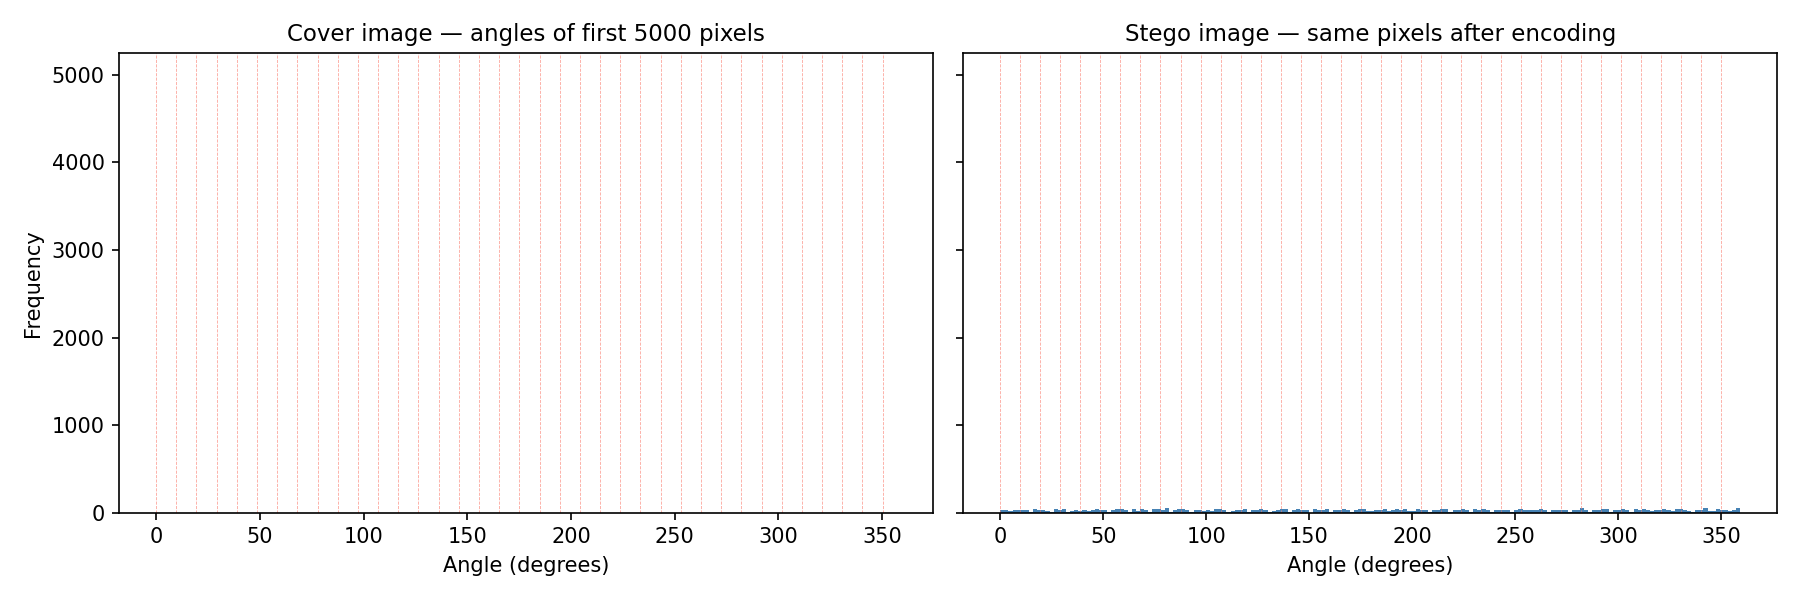
\includegraphics[width=0.95\linewidth]{angle_comparison.png}
    \caption{Angle histogram of the 5000 encoded pixels in the cover (left)
    and stego image (right). Dashed lines mark the 37 nominal token angles.
    The cover histogram reflects the natural angular distribution of the
    image; the stego histogram collapses into 37 narrow peaks aligned with
    the token sectors.}
    \label{fig:angle_comparison}
\end{figure}

The cover image's angle distribution is broad and irregular, reflecting the
diversity of color transitions in a natural scene. After encoding, the same
pixels exhibit 37 sharply defined peaks. This contrast is detectable by any
steganalyst who applies an angular distribution test to the RG vector field.

\subsection{Polar Distribution}

Figure~\ref{fig:polar_comparison} presents the same data as polar scatter
plots.

\begin{figure}[H]
    \centering
    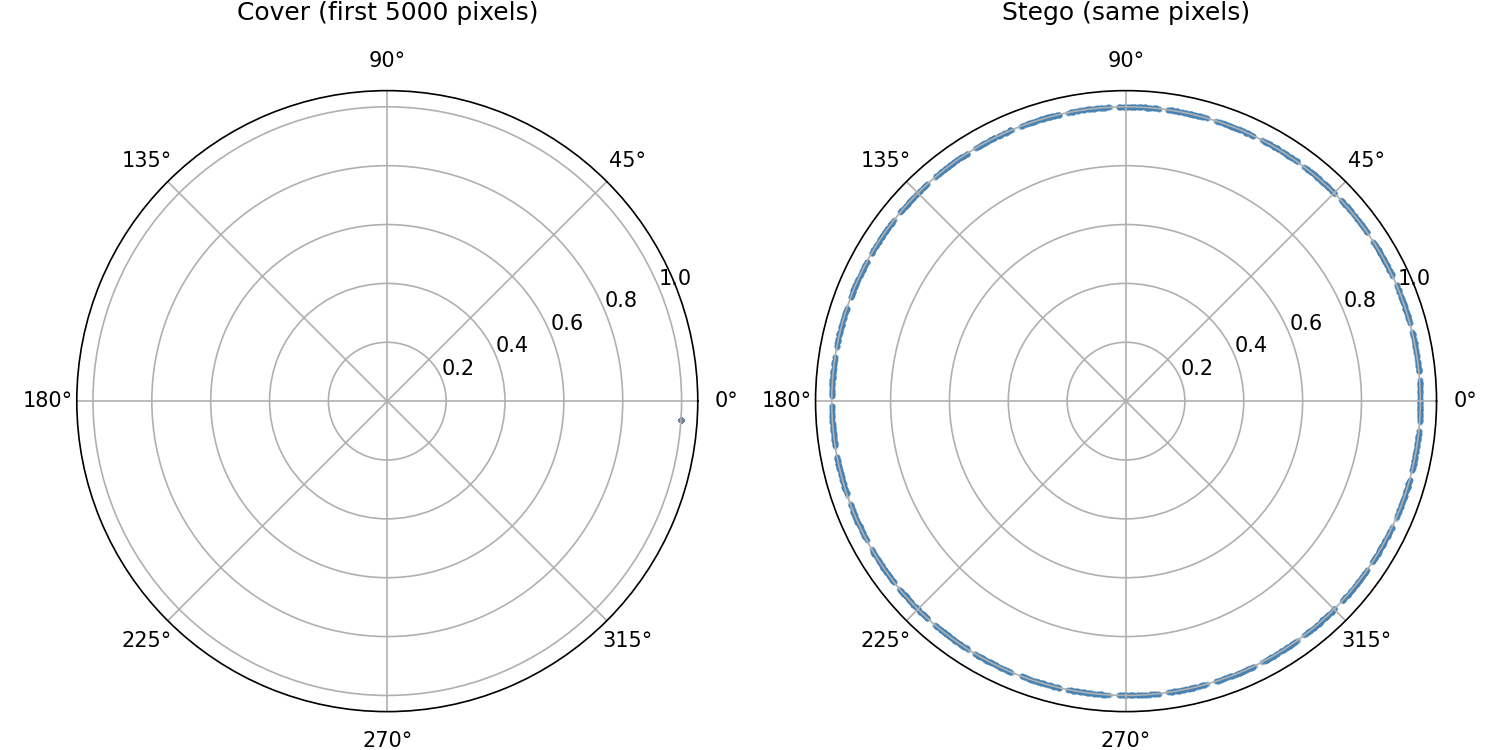
\includegraphics[width=0.85\linewidth]{polar_comparison.png}
    \caption{Polar scatter plot of vector angles for the 5000 encoded pixels.
    Left: cover image, showing a diffuse natural distribution. Right: stego
    image, showing 37 radial spokes at equal angular intervals --- the
    geometric fingerprint of the encoding scheme.}
    \label{fig:polar_comparison}
\end{figure}

The 37-spoke pattern in the stego polar plot has no analogue in natural
image statistics and constitutes a strong anomaly signal detectable without
knowledge of the encoding scheme, vocabulary, or message content.

\subsection{Perceptual Distortion}

Figure~\ref{fig:distortion} shows the distribution of per-pixel Euclidean
distortion $\|(R_j', G_j') - (R_j, G_j)\|_2$ over the 5000 modified
pixels.

\begin{figure}[H]
    \centering
    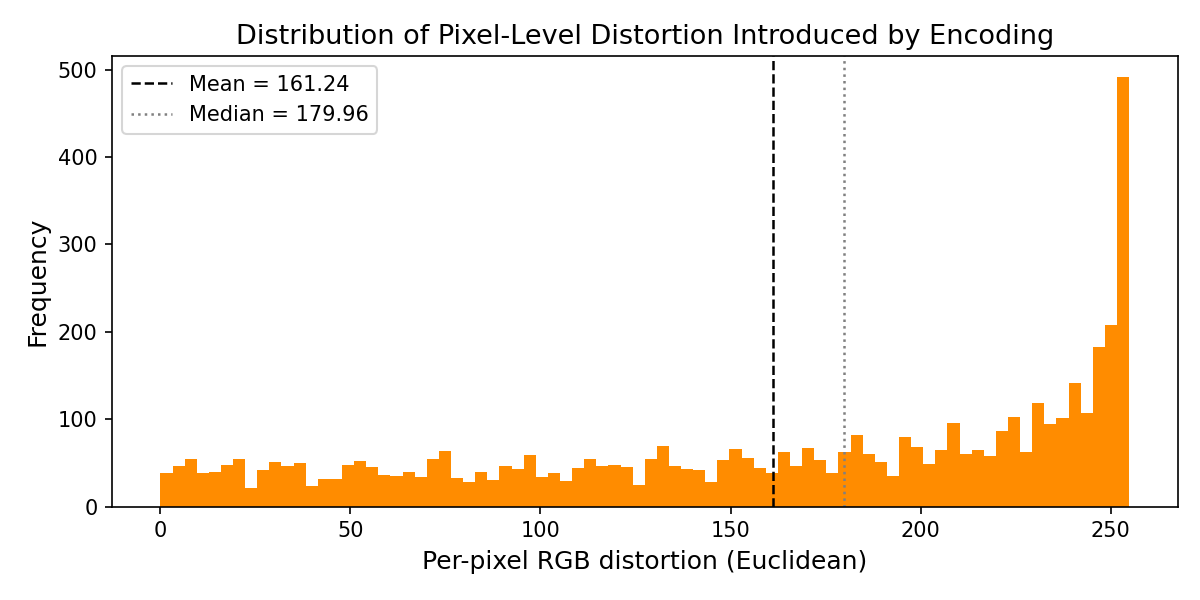
\includegraphics[width=0.72\linewidth]{distortion.png}
    \caption{Per-pixel RGB distortion introduced by encoding across 5000
    pixels. Pixels whose original direction was already near the target
    sector experience low distortion; pixels pointing far from the target
    are rotated substantially.}
    \label{fig:distortion}
\end{figure}

Distortion is heterogeneous: pixels already close to the target angular
sector are rotated by a small angle and incur low distortion, while pixels
pointing far from the target sector incur large color shifts. This means
the perceptual impact of encoding is spatially non-uniform and depends
on both the message content and the cover image's local color structure.

\subsection{Magnitude Preservation}

Figure~\ref{fig:magnitude_scatter} shows original vector magnitude $r_j$
against encoded magnitude $r_j'$ for the 5000 modified pixels.

\begin{figure}[H]
    \centering
    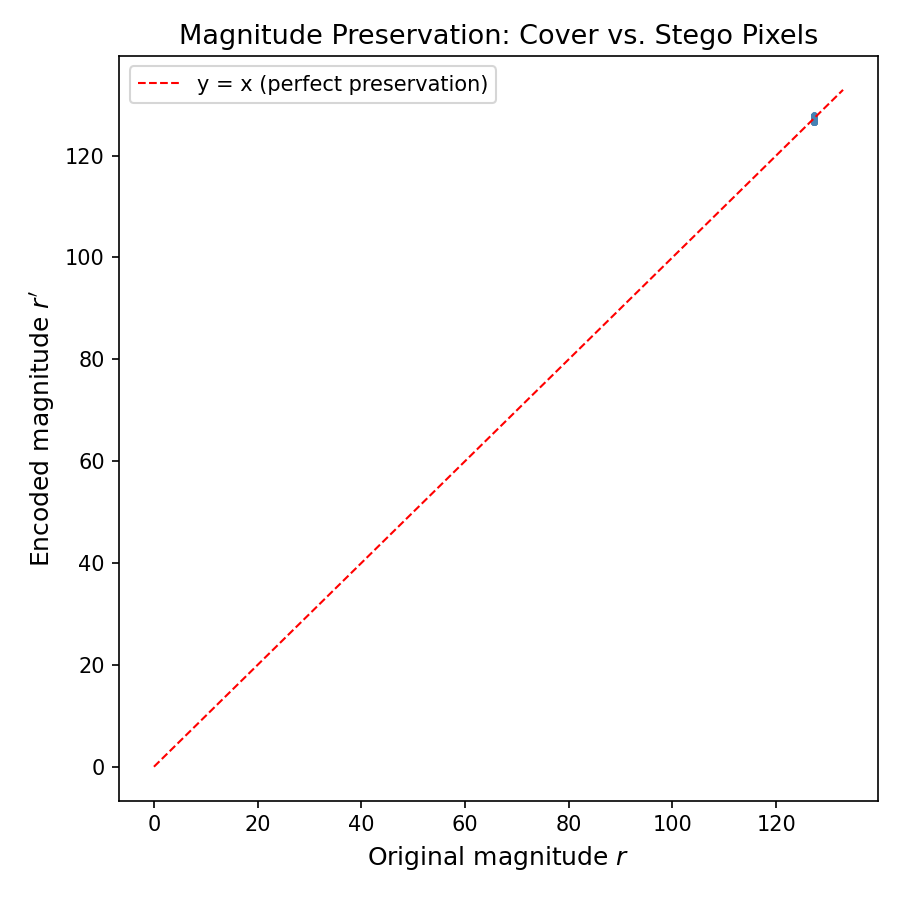
\includegraphics[width=0.60\linewidth]{magnitude_scatter.png}
    \caption{Original vs.\ encoded vector magnitude for 5000 pixels. Points
    near the $y = x$ diagonal confirm that magnitude preservation is
    effective for pixels with $r_j \geq r_{\min} = 30$. Points at
    $r_j' = 30$ for small $r_j$ reflect the magnitude floor applied to
    near-gray pixels.}
    \label{fig:magnitude_scatter}
\end{figure}

Points cluster tightly along the $y = x$ diagonal for $r_j \geq 30$,
confirming that encoding does not systematically alter pixel brightness.
The cluster at $r_j' = 30$ corresponds to near-gray pixels pushed outward
by the magnitude floor.

\subsection{Comparison with LSB Encoding}

Table~\ref{tab:comparison} summarizes key properties of LSB substitution
and the proposed method.

\begin{table}[H]
    \centering
    \caption{LSB substitution vs.\ angular direction encoding.}
    \label{tab:comparison}
    \begin{tabular}{lcc}
        \toprule
        \textbf{Property} & \textbf{LSB} & \textbf{Angular (Ours)} \\
        \midrule
        Embedding domain        & Amplitude       & Direction (angle) \\
        Bits per pixel          & 1--3            & $\approx 5.2$ \\
        Requires cover image    & Yes             & Yes \\
        B channel modified      & Yes             & No \\
        Magnitude preserved     & No              & Yes \\
        Primary distortion      & Intensity $\pm1$ & Color rotation \\
        Detected by             & Pair histograms, RS & Angle histograms \\
        \bottomrule
    \end{tabular}
\end{table}

% ─────────────────────────────────────────────────────────────────────────────
\section{Proposed Extensions}
\label{sec:extensions}

\subsection{Differential Angular Encoding}

The detectability weakness of Section~\ref{sec:experiments} is specific to
absolute direction encoding: every token maps to a fixed angular sector, so
the stego angle distribution always exhibits the same 37-spoke pattern
regardless of message content.

Differential encoding removes this by encoding the angular change between
consecutive pixels rather than the absolute angle. Let $\theta_0 \in
[0°, 360°)$ be a secret reference angle used as the key. The encoding rule
for the $i$-th token $t_{k_i}$ is:
\[
    \theta_i = \theta_{i-1} + k_i \cdot \Delta\phi + \varepsilon_i
               \pmod{360°},
\]
and decoding recovers the increment:
\[
    \hat{k}_i = \left\lfloor
        \frac{\theta_i - \theta_{i-1}}{\Delta\phi}
    \right\rceil \pmod{37}.
\]
Because $\theta_0$ is drawn uniformly and each subsequent $\theta_i$ is an
accumulated sum of uniform-modular increments, the marginal distribution of
each $\theta_i$ converges to uniform over $[0°, 360°)$ by equidistribution
of random walks on $\mathbb{Z}/N\mathbb{Z}$. The 37-spoke signature
vanishes. Without $\theta_0$, an attacker cannot recover the first or any
subsequent token, so the scheme simultaneously solves detectability and
introduces a cryptographic key.

\subsection{Spherical Encoding}

The current method uses only two of the three color channels, treating B as
a free variable. A natural generalization interprets the full centered triple
$(R{-}128,\,G{-}128,\,B{-}128)$ as a point on a sphere of radius $r$ in
$\mathbb{R}^3$, parameterized by spherical coordinates $(\phi, \lambda)$:
\begin{align*}
    R - 128 &= r\sin\phi\cos\lambda, \\
    G - 128 &= r\sin\phi\sin\lambda, \\
    B - 128 &= r\cos\phi,
\end{align*}
where $\phi \in [0°, 180°]$ and $\lambda \in [0°, 360°)$. A vocabulary of
$N$ tokens is mapped to $N$ near-uniformly distributed points on the unit
sphere using a Fibonacci lattice. Encoding sets $(\phi, \lambda)$ to the
spherical coordinates of the target token while preserving $r$; decoding
identifies the nearest codebook point by great-circle distance.

Three advantages follow from this generalization. First, capacity increases
roughly quadratically with angular resolution: the sphere accommodates
$O((\Delta\phi)^{-2})$ tokens versus $O((\Delta\phi)^{-1})$ on the circle,
making a 128-character ASCII vocabulary feasible with greater inter-token
separation than the 2D scheme. Second, all three channels are modified,
distributing distortion across the full RGB triple. Third, the natural
distribution of 3D color vectors in photographic images is less well
characterized than the 2D RG distribution, making the detection of a
spherical fingerprint a substantially harder problem for a steganalyst.

% ─────────────────────────────────────────────────────────────────────────────
\section{Discussion}
\label{sec:discussion}

\subsection{Detectability}

The angle histogram and polar plot analyses confirm that absolute angular
encoding introduces an unmistakable geometric fingerprint in the stego
image. The 37-spoke pattern is absent from natural images and detectable
without any knowledge of the encoding alphabet, token count, or message.
An attacker who computes the $(R{-}128, G{-}128)$ angles of suspected pixels
and plots their distribution can detect the presence of an embedded message
with high confidence.

This weakness is not intrinsic to direction-based encoding; it is a
consequence of the fixed mapping from tokens to absolute angular sectors.
Differential encoding eliminates fixed-sector clustering; spherical encoding
disperses the fingerprint into a harder-to-characterize three-dimensional
space.

\subsection{Perceptual Distortion and the Role of Cover Image Choice}

Magnitude preservation limits brightness changes but does not bound the hue
shift, which is determined by the angular distance between a pixel's
original direction and the target token sector. In the worst case, a
saturated pixel pointing near $0°$ encoded to a token near $180°$ will
undergo a nearly complementary hue shift while maintaining its brightness.
Whether this produces a visible artifact depends on the local image context.

A practical mitigation is adaptive pixel selection: prefer pixels whose
original direction already falls near the target token sector, incurring
minimal rotation. This lowers mean distortion without altering the encoding
or decoding logic. A more aggressive version would order message characters
by the token sector, selecting pixels from image regions that naturally point
in the required direction.

\subsection{Robustness}

The scheme shares the robustness limitations of all spatial-domain
steganography: JPEG compression, resizing, or color space conversion shifts
vector angles unpredictably and corrupts the embedded message. Adding an
error-correcting code to the message prior to encoding would provide
robustness against moderate per-pixel perturbations without modifying the
angular encoding mechanism.

% ─────────────────────────────────────────────────────────────────────────────
\section{Conclusion}
\label{sec:conclusion}

We have presented a cover-image steganographic scheme that embeds text by
rotating the directional component of color vectors in the RG plane while
preserving vector magnitudes. The method encodes approximately 5.2 bits per
pixel, modifies only two of three color channels, and produces lossless
decoding on natural images for the noise and magnitude parameters chosen.

The primary limitation is detectability: absolute angular encoding collapses
the angle distribution of modified pixels into 37 narrow peaks at regular
intervals, a signature that is absent from natural image statistics and
detectable without knowledge of the encoding scheme. We have quantified this
through comparative histogram and polar-plot analysis and have characterized
the per-pixel distortion through PSNR and Euclidean distance measurements.

Two extensions are proposed to address the detectability problem. Differential
encoding accumulates angular increments to produce a uniform angle
distribution and doubles as a stream cipher. Spherical encoding generalizes
the scheme to all three color channels, increasing vocabulary capacity and
distributing the angular fingerprint into a higher-dimensional space that is
harder to analyze. Implementing, evaluating, and comparing these extensions
against the baseline scheme is the primary direction for future work.

% ─────────────────────────────────────────────────────────────────────────────
\bibliographystyle{plain}
\bibliography{refs}

\end{document}